%iffalse
\let\negmedspace\undefined
\let\negthickspace\undefined
\documentclass[journal,12pt,onecolumn]{IEEEtran}
\usepackage{cite}
\usepackage{amsmath,amssymb,amsfonts,amsthm}
\usepackage{algorithmic}
\usepackage{graphicx}
\usepackage{textcomp}
\usepackage{xcolor}
\usepackage{txfonts}
\usepackage{listings}
\usepackage{enumitem}
\usepackage{mathtools}
\usepackage{gensymb}
\usepackage{comment}
\usepackage[breaklinks=true]{hyperref}
\usepackage{tkz-euclide} 
\usepackage{listings}
\usepackage{gvv}                                        
%\def\inputGnumericTable{}                                 
\usepackage[latin1]{inputenc}     
\usepackage{xparse}
\usepackage{color}                                            
\usepackage{array}                                            
\usepackage{longtable}                                       
\usepackage{calc}                                             
\usepackage{multirow}
\usepackage{multicol}
\usepackage{hhline}                                           
\usepackage{ifthen}                                           
\usepackage{lscape}
\usepackage{tabularx}
\usepackage{array}
\usepackage{float}
\newtheorem{theorem}{Theorem}[section]
\newtheorem{problem}{Problem}
\newtheorem{proposition}{Proposition}[section]
\newtheorem{lemma}{Lemma}[section]
\newtheorem{corollary}[theorem]{Corollary}
\newtheorem{example}{Example}[section]
\newtheorem{definition}[problem]{Definition}
\newcommand{\BEQA}{\begin{eqnarray}}
\newcommand{\EEQA}{\end{eqnarray}}
\usepackage{float}
\usepackage{listings}
\usepackage{xcolor}
%\newcommand{\define}{\stackrel{\triangle}{=}}
\theoremstyle{remark}
\usepackage{ circuitikz }
%\newtheorem{rem}{Remark}
% Marks the beginning of the document
\begin{document}
\title{8.1.1.Ex 1}
\author{EE24BTECH11016 - DHWANITH M DODDAHUNDI}
\maketitle
\renewcommand{\thefigure}{\theenumi}
\renewcommand{\thetable}{\theenumi}
\parindent 0px \textbf{Question:} Find the area enclosed by the circle $x^{2}+y^{2}=a^{2}$.\\
\solution\\
\textbf{Theoretical Solution:}\\
Finding Area
\begin{align}
    A&=4\int^{a}_{0}ydx
\end{align}
Since $x^{2}+y^{2}=a^{2}$ ,we get $y=\pm \sqrt{a^{2}-x^{2}}$
\begin{align}
        A&=4\int^{a}_{0}\sqrt{a^{2}-x^{2}}dx \\  
        A&=4\sbrak{\frac{x}{2}\sqrt{a^{2}-x^{2}}+\frac{a^{2}}{2} \sin^{-1}{\brak{\frac{x}{a}}}}^a_0\\
                A&=4\sbrak{\frac{a}{2}\times 0 +\frac{a^{2}}{2} \sin^{-1}{\brak{1}}-0}\\
                A&=4\brak{\frac{a^{2}}{2}}\brak{\frac{\pi}{2}} \\
                A&=\pi a^{2}
\end{align}

\textbf{Computational Solution:}\\
Using the trapezoidal rule to get the area\\
The trapezoidal rule is as follows.
\begin{align}
    A &= \int_a^b f\brak{x}\, dx \approx h\brak{\frac{1}{2}f\brak{a} + f\brak{x_1} + f\brak{x_2} \cdots + f\brak{x_{n-1}} + \frac{1}{2}f\brak{b}}\\
    h &= \frac{b-a}{n}\\
    A &= j_n, \text{ where, } j_{i + 1} = j_i + h\frac{f\brak{x_{i+1}} + f\brak{x_i}}{2}\\ 
        \xrightarrow{} j_{i + 1} &= j_i + h\brak{\sqrt{x_{i+1}}+\sqrt{x_{i}}}\\
    x_{i+1} &= x_i + h\\
    h&=\frac{1}{30000}\\
    n&=30000
\end{align}
Using the code answer obtained is $A=3.141592427302344$ sq. units for a radius of 1 unit.
\begin{figure}[ht]
    \centering
    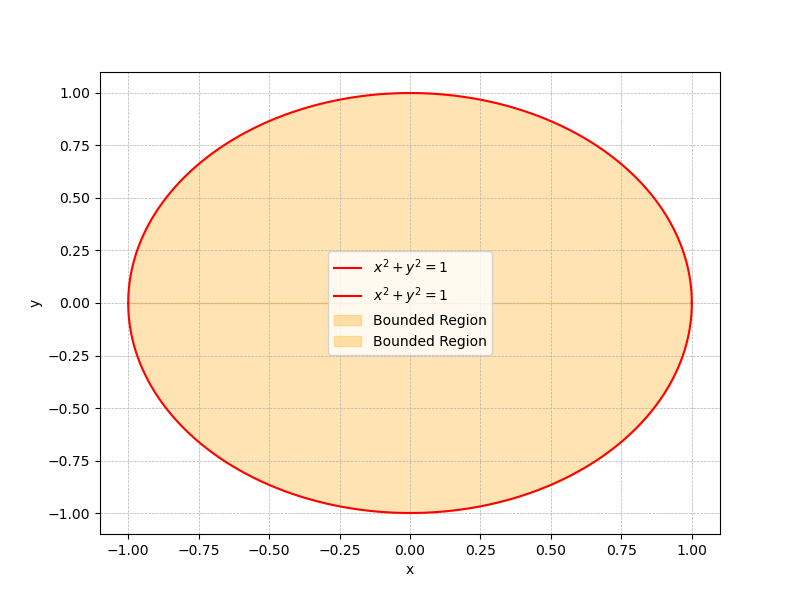
\includegraphics[width=\columnwidth]{figs/fig_circle.png}
 \end{figure}
\end{document}

